\documentclass[fleqn]{jbook}
\usepackage{physpub}

\begin{document}

\begin{question}{専攻 問題4}{}

図1のような装置によって、標的中に、負ミュオン($\mu^-$)を静止させると、
ミュー原子($\mu^-$が原子核のクーロン場に束縛された原子)が生成される。
生成当初、$\mu^-$はミュー原子の高い励起状態にあるが、$10^{-12}$秒程度
の短時間にX線などを出して基底状態に落ちる。これに関連し、以下の問に
答えよ。ただし、簡単のために、電子の影響は無視して良い。つまり、
ミュー原子は、原子核の回りに負ミュオンが一個だけまわっている
「水素様原子」とみなせるものとする。なお、必要に応じて、以下の数値を
参照せよ。
\[
\begin{array}{ll}
  m_e   \,\mbox{(電子質量)}    = 0.511\Unit{MeV/c^2}	&%
  \mbox{水素原子の1s電子の束縛エネルギー} = 13.6 \Unit{eV} \\
  m_\mu \,\mbox{(ミュオン質量)}= 106  \Unit{MeV/c^2}    &%
  \mbox{ボーア半径} = 0.529 \Keta{-10} \Unit{m} \\
  m_p   \,\mbox{(陽子質量)}    = 938  \Unit{MeV/c^2}	&\\%
\end{array}
\]

\begin{center}
  \mbox{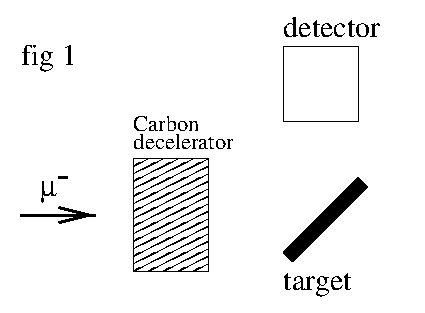
\includegraphics[clip]{1995phy4-1.eps}}\hspace{5mm}%
  \mbox{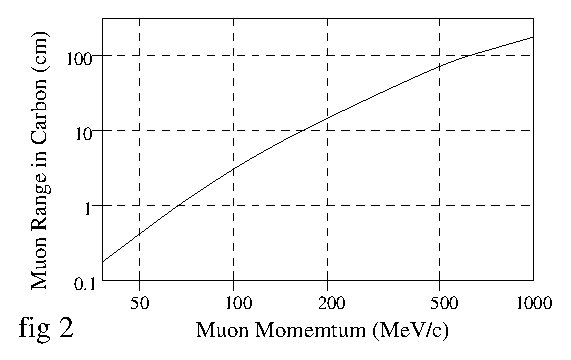
\includegraphics[clip]{1995phy4-2.eps}}
\end{center}


\begin{subquestions}
\SubQuestion
  \underline{運動エネルギー}$120$MeVの$\mu^-$を図1のように炭素の板に
  よって減速し、薄い標的に静止させたい。炭素板の厚さをどの様に選べば
  よいか。図2のグラフを参考にして概算せよ。但し、図2はミュオンの炭素
  中での飛程を、入射粒子の\underline{運動量}の関数で示したものである。

\SubQuestion
  ある単元素標的を用い、図1の装置でミュー原子が励起状態から基底状態に
  向かって次々に遷移する際に放出されるX線を測定したところ、図3のよう
  なエネルギースペクトルが得られた。図中に強く見えているピークのうち、
  Bのピークは、$\mu^-$原子の3d$\rightarrow$ 2p遷移によるものであると
  いう。図中のA,Cのピークは、各々どの様な遷移によるものか。推測せよ。
  (注:ミュー原子のX線遷移は、3d$\rightarrow$ 2pの様に、主として電気
  双極子遷移であることが知られている。)\\
%
\parbox[t]{60mm}{
\SubQuestion
  図3のデータをもとに、標的の原子番号$Z$を推定せよ。

\SubQuestion
  標的核が原子番号$Z=82$、質量数$A=208$である場合、核を点電荷とみなし
  て、ミュー原子の1s軌道半径を概算し、これを標的核半径と比較せよ。

\SubQuestion
  実際には原子核は点電荷ではなく、有限の核半径を持つ。この効果が、図3
  の様なスペクトルにどの様に現れるかを、簡潔に論じよ。
}\parbox[t]{100mm}{
\begin{center}
  \mbox{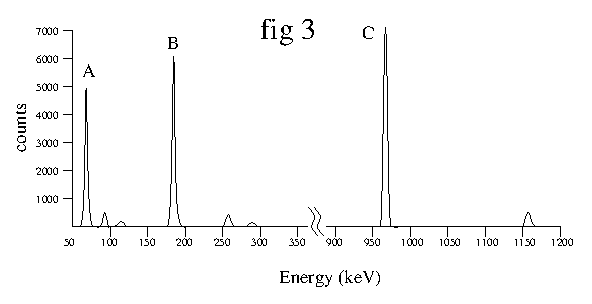
\includegraphics[clip]{1995phy4-3.eps}}
\end{center}}

\end{subquestions}


\end{question}
\begin{answer}{専攻 問題4}{}

\begin{subanswers}
\SubAnswer
  何cmの厚さの炭素減速材を使えば入射粒子の運動エネルギーをすべて
  奪えるかを考える。運動エネルギーを $T$とすると、
%
  \[ T = E - m c^2 = \sqrt{(mc^2 )^2 + (pc)^2} - mc^2 \]
%
  これより
%
  \[ pc = \sqrt{(T+mc^2)^2 - (mc^2)^2} \approx 200 \Unit{MeV} \]
%
  よって図2より、$17\Unit{cm}$の炭素減速材を用いればよい。


\SubAnswer
  電気双極子遷移のみを考えればよいので、主量子数と方位量子数が1減少
  する遷移を考える。このとき、X線スペクトルのエネルギー $E$ は、
  遷移先の準位の主量子数を$n$として
%
  \[ E \propto \left(\frac{1}{n^2} - \frac{1}{(n+1)^2} \right) \]
%
  で表される。ただし、量子欠損は考えていない。\\
%
  A,B のスペクトルの主量子数を$n_A,n_B$として、エネルギー$E_A, E_B$
  の比は、
%
  \[ \frac{E_A}{E_B} = \frac{\frac{1}{n_A^ 2} - \frac{1}{(n_A +1)^2}}%
     {\frac{1}{n_B^2} - \frac{1}{(n_B+1)^2} } \]
%
  となる。

  $n_B=2$ と図3のデータから計算して$n_A=3$ と分かる。

  与えられた遷移が 3d $\rightarrow$ 2p の遷移なので、 Aは、 3dへ
  落ちる遷移でなくてはならない。よって、Aは 4f$\rightarrow$ 3d の
  遷移である。

  Cは、もっとも大きなエネルギーのピークであることと、2pから落ちる
  遷移がなくてはならないことから、2p $\rightarrow$ 1s の遷移である。



\SubAnswer
  ボーアモデルでは、電子のエネルギー準位 $E_n$は
%
  \[ E_n \propto \frac{Z^2 m_e}{n^2} \]
%
  である。ボーアモデルをミュー原子に適応する。$Z=1$、$n=1$の水素原子の
  1s状態の電子の束縛エネルギーが$13.6\Unit{eV}$であることを利用して
  負ミュオンのエネルギー準位 $E_n$は
%
  \[ E_n = \frac{Z^2}{n^2}\frac{m_\mu}{m_e} \times 13.6 \Unit{eV} \]
%
  となる。$Z$ を決めるに当たって B の遷移を使う。
%
  \[ 190 \Keta{3} = \left( \frac{1}{2^2} - \frac{1}{3^2} \right)%
                    \times \frac{106}{0.511} \times 13.6 \times Z^2 \hspace{15mm}%
               \Yueni Z \approx 22 \]
%
  よって標的の原子番号は 22(Ti) と予想される。



\newpage
\SubAnswer
  ボーアモデルでは電子の軌道半径 $r_n$ は
%
  \[ r_n \propto \frac{n^2}{Z m_e} \]
%
  である。前問と同様にこれをミュー原子に適応する。水素原子の1s電子の
  軌道半径の期待値が $a_B$であることから、ミュー原子の 1s軌道半径は
  $Z=82$なので
%
  \[ r = \frac{m_e}{Zm_\mu} a_B \approx 3.11 \Keta{-15}\Unit{m} \]
%
  となる。

  標的核半径は、質量数と原子核の半径との間の関係式
%
  \[ r_N \approx 1.3 \Keta{-15} \times A^\frac{1}{3} \Unit{m} \]
%
  を用いて、
%
  \[ r_N \approx 7.70 \Keta{-15}\Unit{m} \]
%
  となるので、ミュー原子の 1s軌道半径の方が小さい。


\SubAnswer
  ミュー原子の原子核の半径が1s軌道半径よりも大きいため、ミュオン
  が感じる中心の原子核の電荷は実際の電荷よりも小さい。なので、中心が
  点電荷であると仮定した場合よりもミュオンの1sエネルギーは不安定に
  なる。つまり高くなる。2p軌道との準位差が縮まるので生成されるX線の
  エネルギーは低くなる。よって図3 のようなスペクトルのピークの位置は
  左に移動する。

  また、クーロン相互作用の場合の、主量子数が同じで軌道運動量の同じ状態の偶然縮退  がとける。当然原子中の電子との相互作用も縮退をとくように働くが、$\mu$粒子の軌道は充分内側なので、それらはあまり影響しないと考えられる。
\end{subanswers}
\end{answer}


\end{document}
